\documentclass{article}
\usepackage{graphicx, amsmath, amsfonts, tikz} % Required for inserting images
\usepackage{caption,float}
\usepackage[style=apa, sorting=nyt]{biblatex}
\addbibresource{repbib.bib}

\newtheorem{remark}{Remark}[section]
\newcommand{\partder}[2]{\dfrac{\partial {#1}}{\partial {#2}}}
\newcommand{\partders}[2]{\dfrac{\partial^2 {#1}}{\partial {#2}^2}}
\newcommand{\abs}[1]{\left| {#1} \right|}
\newcommand{\paren}[1]{\left( {#1} \right)}
\newcommand{\E}[1]{E\left[ {#1} \right]}
\newcommand{\Var}[1]{\text{Var}\left[ {#1} \right]}
\newcommand{\grad}[1]{\text{grad}\left[ {#1} \right]}
\newcommand{\var}[1]{\text{Var}\left( {#1} \right)}
\newcommand{\norm}[1]{\left| \left | {#1} \right| \right|}
\newcommand{\R}{\mathbb{R}}
\newcommand{\dyx}{\dfrac{d y}{d x}}
\newcommand{\der}[2]{\dfrac{d {#1}}{d {#2}}}
\newcommand{\inner}[2]{\langle {#1},{#2}}
\newcommand{\Lag}{\mathcal{L}}
\newcommand{\asto}{\overset{as}{\to}}
\newcommand{\pto}{\overset{p}{\to}}
\newcommand{\dto}{\overset{d}{\to}}
\newcommand{\Bx}{B_{\varepsilon}(x)}
\newcommand{\plim}{\mathop{\text{plim}}\limits}
\newcommand{\argmax}{\mathop{\text{argmax}}\limits}
\newcommand{\ubar}[1]{\text{\b{$#1$}}}

\title{bargaining power}
\author{}
\date{Last modification: \today}

\begin{document}

\maketitle
\section{The Model}
%=======================================
\subsection{Basic Setup}\label{subsec:setup}
%=======================================
Time is discrete, indexed by $t = 0,1,2,\dots$. A risk-neutral principal and a risk-averse agent interact repeatedly. Within each period, the timing is as follows: at $t=0$ the public state is observed, the parties bargain over one-period contracts, the agent chooses effort after the contract is signed, and output is then realized and the transfer paid. This timing is essential for the moral hazard problem and is discussed formally in Remark \ref{rem:renegotiation}. In each period, the agent supplies effort $a_t \in \mathbb{R}_+$ and stochastic output is realized according to
\[
y_t = \theta a_t + \sigma \varepsilon_t, \qquad \varepsilon_t \sim \mathcal{N}(0,1),
\]
where $\varepsilon_t$ is an i.i.d.\ production shock, $\theta > 0$ is productivity, and $\sigma > 0$ is output volatility. The agent incurs cost $c(a_t) = \frac{k}{2}a_t^2$ with $k > 0$, and she has CARA utility $u(w) = -\exp(-\gamma w)$ with risk aversion $\gamma > 0$. The principal is risk neutral and he maximizes expected profit $\Pi = \mathbb{E}[y - w]$. Both parties discount future payoffs at rate $\rho \in (0,1)$.

\textcite{holmstrom1987} show that with CARA preferences and normally distributed output, optimal contracts are linear in output. We therefore restrict attention to contracts of the form
\[
w_t = \alpha_t + \beta_t y_t,
\]
where $\alpha_t \in \mathbb{R}$ is the fixed payment and $\beta_t \in [0,1]$ is the performance-based slope. Under this contract, the agent's certainty equivalent, measured in monetary units, is
\[
\text{CE}_t = \alpha_t + \beta_t \theta a_t - \frac{\gamma}{2}\beta_t^2 \sigma^2 - \frac{k}{2}a_t^2,
\]
and the principal's expected payoff, also in monetary units, is
\[
\Pi_t = (1-\beta_t)\theta a_t - \alpha_t.
\]
Because CARA utility admits a monetary certainty equivalent representation, the agent's payoff and the principal's profit are expressed in the same units and can be added directly. Total surplus is therefore
\[
S_t = \text{CE}_t + \Pi_t = \theta a_t - \frac{\gamma}{2}\beta_t^2 \sigma^2 - \frac{k}{2}a_t^2.
\]
The fixed payment $\alpha_t$ is a pure transfer: it increases the agent's certainty equivalent by one unit and decreases the principal's profit by one unit, leaving total surplus unchanged.

%=======================================
\subsection{Symmetric information benchmark}\label{subsec:symmetric}
%=======================================

We first characterize optimal effort and payoffs when the principal observes effort directly, so no incentive constraint is required. The principal specifies $a_t$ directly in the contract and chooses it to maximize total surplus under symmetric information:
\[
\max_{a_t} S_t(a_t) = \theta a_t - \frac{\gamma}{2}\beta_t^2 \sigma^2 - \frac{k}{2}a_t^2.
\]
The first-order condition with respect to $a_t$ is
\[
\theta - k a_t = 0 \quad \implies \quad a_t^{\text{FB}} = \frac{\theta}{k}.
\]
This is the first-best effort level. It is determined solely by the ratio of productivity to the cost parameter and is independent of the incentive slope $\beta_t$: since effort is contractible, the principal can implement $a_t^{\text{FB}}$ with any value of $\beta_t$, adjusting $\alpha_t$ to achieve any desired division of surplus.

The efficient risk-sharing arrangement minimizes the agent's risk premium, given by $\frac{\gamma}{2}\beta_t^2\sigma^2$, for a given expected transfer. Since the agent is risk-averse and the principal is risk-neutral, it follows that the principal should bear all output risk. This is a consequence of the difference in risk attitudes: any residual output risk borne by the agent reduces total surplus without improving incentives under symmetric information. The efficient arrangement therefore sets $\beta_t = 0$, so that the general contract $w_t = \alpha_t + \beta_t y_t$ reduces to a fixed wage:
\[
w_t = \alpha_t \quad (\text{no performance pay}).
\]
With first-best effort $a_t^{\text{FB}} = \theta/k$ and full insurance $\beta_t = 0$, total surplus is
\[
S^{\text{FB}} = \theta \left(\frac{\theta}{k}\right) - \frac{k}{2}\left(\frac{\theta}{k}\right)^2 = \frac{\theta^2}{2k}.
\]
The agent's certainty equivalent is $\text{CE}_t = \alpha_t - \theta^2/(2k)$ and the principal's expected payoff is $\Pi_t = \theta^2/k - \alpha_t$. The fixed payment $\alpha_t$ can be adjusted to achieve any division of $S^{\text{FB}}$ between the parties.

Under symmetric information, the optimal arrangement achieves first-best effort $a_t^{\text{FB}} = \theta/k$, full insurance $\beta_t = 0$, and maximum total surplus $S^{\text{FB}} = \theta^2/(2k)$.

%=======================================
\subsection{Asymmetric information: moral hazard}\label{subsec:moral_hazard}
%=======================================

We now assume the principal observes only output $y_t$, not effort $a_t$. The agent chooses effort to maximize the certainty equivalent given the contract, subject to the IC constraint:
\[
a_t \in \arg\max_{a} \left[\alpha_t + \beta_t \theta a - \frac{\gamma}{2}\beta_t^2 \sigma^2 - \frac{k}{2}a^2\right].
\]

\textcolor{olive}{Aclarar por qué aquí no hace falta el first order approach ni sus condiciones de validez, a diferencia de la literatura general de moral hazard}

\textcolor{blue}{
In general moral hazard problems, replacing the agent's incentive compatibility constraint, $a \in \arg\max_a \mathbb{E}[v(w,a)]$, with the first-order condition of that problem is called the first-order approach, and it is only valid under
additional regularity conditions on the family of conditional output distributions $F(y\mid a)$, since the agent's objective need not be concave in $a$ in general \parencite{mirrlees1999}. \textcite{rogerson1985} gives sufficient conditions, the monotone likelihood ratio condition together with the convexity of the distribution function condition (MLRC and CDFC), and \textcite{jewitt1988} provides an alternative, less restrictive set of conditions. \\
Under the CARA-normal-quadratic specification (the same structure used by \textcite{holmstrom1987}), output enters only through a linear shift in the mean of a normal distribution, $y = \theta a + \sigma\varepsilon$, and the cost of effort is quadratic. For any fixed contract $(\alpha,\beta)$, the agent's certainty equivalent
\[
\alpha + \beta\theta a - \frac{\gamma}{2}\beta^2\sigma^2 - \frac{k}{2}a^2
\]
is a strictly concave, twice differentiable function of $a$ alone, since its second derivative is $-k < 0$ for all $a$. The first-order condition $a_t^*(\beta_t) = \beta_t\theta/k$ is therefore both necessary and globally sufficient for the agent's problem, with no need to impose MLRC, CDFC, or any other condition on a family of output distributions. Incentive compatibility reduces to this single substitution throughout the paper. We flag this explicitly because it is the point in the model where the general moral hazard literature usually requires the most care, and it is worth being clear about exactly why that care is unnecessary here.
}

The first-order condition yields
\[
a_t^*(\beta_t) = \frac{\theta}{k}\beta_t .
\]

Effort is now endogenous to the incentive slope. To induce higher effort, the principal must increase $\beta_t$, which exposes the agent to more risk. Note also that effort is increasing in $\beta_t$: a steeper performance-based slope induces greater effort, but at the cost of more risk borne by the agent. Substituting optimal effort into payoffs gives
\[
\text{CE}_t(\alpha_t, \beta_t) = \alpha_t + \left(\frac{ \theta^2}{2k} - \frac{\gamma \sigma^2}{2} \right)\beta^2_t=: \alpha_t + C(\beta_t)
\]
and
\[
\Pi_t(\alpha_t, \beta_t) = \dfrac{\theta^2}{k}(1-\beta_t)\beta_t - \alpha_t =: D(\beta_t) - \alpha_t,
\]
where $C(\beta_t)$ and $D(\beta_t)$ capture the net effects of the slope on each party's payoff, excluding the fixed payment.

Total surplus under moral hazard is
\[
S(\beta_t) = C(\beta_t) + D(\beta_t) = \frac{\beta_t \theta^2}{k} - \frac{\beta_t^2 \theta^2}{2k} - \frac{\gamma}{2}\beta_t^2 \sigma^2.
\]

\textcolor{olive}{Pensar en reescribir esta expresión para sacar un resultado interpretativo sobre las raíces}\\
\textcolor{red}{\[
S(\beta_t)  = \frac{\beta_t \theta^2}{k} - \frac{\beta_t^2 \theta^2}{2k} - \frac{\gamma}{2}\beta_t^2 \sigma^2.
\]}

\textcolor{blue}{
\begin{align*}
    S(\beta_t) &= \frac{ \theta^2}{k} \beta_t -\left[ \frac{ \theta^2}{2k} + \frac{\gamma}{2} \sigma^2\right]\beta_t^2\\
    &=\left(\frac{\theta^2}{k} -\left[\dfrac{\theta^2}{2k}+\dfrac{\gamma}{2}\sigma^2 \right]\beta_t \right)\beta_t
\end{align*}
This factorization shows that $S(\beta_t)$ has two roots in $\beta_t$, namely $\beta_t = 0$ and 
\[
    \beta^{\text{SR}}=\dfrac{2\theta^2/k}{\gamma\sigma^2+\theta^2/k}
\]
}

The efficient slope maximizes $S(\beta_t)$. The first-order condition is
\[
\frac{\theta^2}{k} - \frac{\theta^2}{k} \beta_t - \gamma \sigma^2 \beta_t = 0,
\]
yielding
\[
\beta^{\text{eff}} = \frac{\theta^2/k}{\gamma \sigma^2 + \theta^2/k} \in (0,1).
\]

This reflects the standard trade-off between incentive provision and risk sharing. Note that $\beta^{\text{eff}} < 1$: some insurance is sacrificed to provide incentives.

\textcolor{blue}{
Note that now that we know $\beta^{\text{eff}}\in (0,1)$ we can infer things on the second root of $S(\beta_t)$, note that $\beta^{\text{SR}}=2\beta^{\text{eff}}$, thus it could be that $\beta^{\text{SR}}$ is either greater than, less than or equal to 1, the most interesting case is $\beta^{\text{SR}}<1$, since this means that there are some values of $\beta_t$ that lead to a negative surplus, this would happen if
\begin{align*}
    \dfrac{2\theta^2/k}{\gamma\sigma^2+\theta^2/k}&<1\\
    \dfrac{2\theta^2}{k}&<\gamma\sigma^2+\dfrac{\theta^2}{k}\\
    \dfrac{\theta^2}{k}&<\gamma\sigma^2\\
    \dfrac{\theta^2}{2k}&<\dfrac{\gamma\sigma^2}{2}
\end{align*}
Note that the left side of this inequality is the total surplus in the symmetric information benchmark, and the right side corresponds to the risk premium when $\beta_t=1$. In other words, the condition states that the first-best surplus, the total size of the pie in the frictionless benchmark, is smaller than the risk premium the agent would bear under full residual claimancy. Put differently, even at its best the relationship does not generate enough value to cover the cost of exposing the agent to all of the production risk.
}

With $\beta_t = \beta^{\text{eff}}$, induced effort is
\[
a^{\text{eff}} = \frac{\beta^{\text{eff}} \theta}{k} = \frac{\theta^2/k}{\gamma \sigma^2 + \theta^2/k} \left(\frac{\theta}{k}\right) = \frac{\theta^3/k}{\gamma k \sigma^2 + \theta^2} < a^{\text{FB}} = \frac{\theta}{k}.
\]

Effort is strictly below the first-best level, reflecting the trade-off between incentives and risk sharing.

Total surplus under the efficient contract is
\[
S^{\text{eff}} = S(\beta^{\text{eff}}) = \frac{\theta^2}{2k} \beta^{\text{eff}}.
\]

The efficiency loss relative to symmetric information is
\[
S^{\text{FB}} - S^{\text{eff}} = \frac{\gamma \sigma^2}{2}\beta^{\text{eff}} > 0.
\]

This loss admits two interpretations. The agent bears risk that the risk-neutral principal could absorb at no cost, and effort falls below the first-best level, reducing productive efficiency. Both effects are direct consequences of the incentive constraint. As risk aversion $\gamma$ or volatility $\sigma^2$ increases, $\beta^{\text{eff}}$ decreases, effort falls further below first-best, and the efficiency loss grows. The optimal slope $\beta^{\text{eff}} \in (0,1)$ is strictly interior, induced effort satisfies $a^{\text{eff}} < a^{\text{FB}}$, and the efficiency loss $S^{\text{FB}} - S^{\text{eff}} > 0$ is positive whenever $\gamma\sigma^2 > 0$. Figure \ref{fig:surplus_curve} illustrates the surplus function and the efficiency loss.

The fixed payment $\alpha_t$ remains a free variable that can be adjusted to split surplus $S^{\text{eff}}$ between the parties without affecting efficiency.

\begin{figure}[H]
\centering
\caption{Total surplus $S(\beta_t)$ as a function of the incentive slope under moral hazard. The curve peaks at $\beta^{\text{eff}} \in (0,1)$; the gap to $S^{\text{FB}}$ is the efficiency loss from the risk-incentive trade-off.}
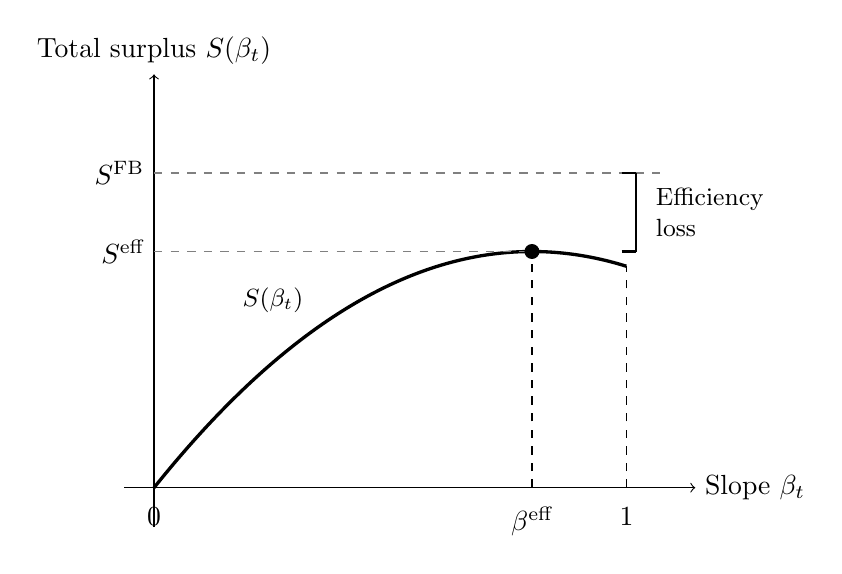
\begin{tikzpicture}[scale=1.25]
    \draw[->] (-0.3,0) -- (5.5,0) node[right] {Slope $\beta_t$};
    \draw[->] (0,-0.4) -- (0,4.2) node[above] {Total surplus $S(\beta_t)$};
    \draw[very thick, black, domain=0:4.8, smooth, variable=\x, samples=80]
        plot ({\x}, {6*(\x/4.8) - 3.75*(\x/4.8)^2});
    \draw[dashed, black] (3.84,0) -- (3.84,2.4);
    \node[below] at (3.84,-0.1) {$\beta^{\text{eff}}$};
    \draw[dashed, black] (4.8,0) -- (4.8,2.25);
    \node[below] at (4.8,-0.1) {$1$};
    \node[below] at (0,-0.1) {$0$};
    \draw[dashed, gray] (0,2.4) -- (3.84,2.4);
    \node[left] at (0,2.4) {$S^{\text{eff}}$};
    \draw[dashed, gray, thick] (0,3.2) -- (5.2,3.2);
    \node[left] at (0,3.2) {$S^{\text{FB}}$};
    \draw[thick, black] (4.9,2.4) -- (4.9,3.2);
    \draw[thick, black] (4.75,2.4) -- (4.9,2.4);
    \draw[thick, black] (4.75,3.2) -- (4.9,3.2);
    \node[right, font=\small, align=left] at (5.0, 2.8) {Efficiency\\loss};
    \filldraw[black] (3.84,2.4) circle (2pt);
    \node[right, font=\small] at (0.8,1.9) {$S(\beta_t)$};
\end{tikzpicture}
\caption*{Source: Own elaboration.}
\label{fig:surplus_curve}
\end{figure}
\vspace{-0.1cm}

%=======================================
\subsection{Optimal contracting benchmark: principal as designer}\label{subsec:variante_B}
%=======================================

We now characterize the contract that emerges when the principal has full bargaining power and designs the contract unilaterally, anticipating the agent's incentive response. This benchmark corresponds to the standard optimal contracting environment of \textcite{holmstrom1979} and \textcite{holmstrom1987}, and will later be shown to coincide with the limiting case $\delta \to 0$ of the Nash bargaining solution of Section \ref{subsec:nash}.

The principal chooses the contract $(\alpha_t, \beta_t)$ to maximize his own payoff, subject to the agent's participation constraint. The incentive compatibility constraint is already embedded in the payoff functions through the substitution $a_t^* = \beta_t\theta/k$, exactly as in Section \ref{subsec:moral_hazard}, so it does not appear as a separate constraint here. The problem is

\[
\max_{\alpha_t,\,\beta_t} \;\; \Pi_t(\alpha_t,\beta_t) = D(\beta_t) - \alpha_t
\]
\[
\text{s.t.} \quad \text{CE}_t(\alpha_t,\beta_t) = \alpha_t + C(\beta_t) \geq \overline{\text{CE}},
\]

where, recall from Section \ref{subsec:moral_hazard},
\[
C(\beta_t) = \frac{\beta_t^2\theta^2}{2k} - \frac{\gamma}{2}\beta_t^2\sigma^2, \qquad D(\beta_t) = \frac{\beta_t\theta^2}{k}(1-\beta_t) = \frac{\beta_t\theta^2}{k} - \frac{\beta_t^2\theta^2}{k}.
\]

Let $\mu \geq 0$ denote the multiplier on the participation constraint. The Lagrangian is

\textcolor{olive}{Poner el Lagrangiano en términos del Teorema 18.3 de \textcite{simon1994mathematics}}
\textcolor{red}{
\[
\mathcal{L}(\alpha_t,\beta_t,\mu) = D(\beta_t) - \alpha_t + \mu\big[\alpha_t + C(\beta_t) - \overline{\text{CE}}\big].
\]
}
\textcolor{blue}{
\begin{align*}
    \Lag(\alpha_t,\beta_t,\mu)&=D(\beta_t)-\alpha_t- \mu\left[ -\text{CE}_t(\alpha_t,\beta_t)+\overline{\text{CE}}\right]\\
    &=D(\beta_t)-\alpha_t + \mu\left[\text{CE}_t(\alpha_t,\beta_t) - \overline{\text{CE}}\right]
\end{align*}
Differentiating with respect to $\alpha_t$ term by term,
\begin{align*}  
    \partder{\Lag}{\alpha_t}&= \partder{}{\alpha_t}\left[ \dfrac{\theta^2}{k}(1-\beta_t)\beta_t - \alpha_t + \mu\left( \alpha_t + \left(\frac{ \theta^2}{2k} - \frac{\gamma \sigma^2}{2} \right)\beta^2_t - \overline{\text{CE}}\right) \right]\\
    &=-1+\mu
\end{align*}
}

Setting this equal to zero,
\[
-1 + \mu = 0 \quad \implies \quad \mu = 1.
\]

The fixed payment $\alpha_t$ enters the principal's payoff with coefficient $-1$ and the constraint with coefficient $+1$, since $\alpha_t$ is a pure one-to-one transfer between the two parties. Relaxing the agent's participation constraint by one unit allows the principal to reduce $\alpha_t$ by exactly one unit, raising his own payoff by exactly one unit. There is no friction in this transfer, so the shadow value of relaxing the constraint is exactly one, not merely positive.

The Karush-Kuhn-Tucker conditions require
\[
\mu\big[\alpha_t + C(\beta_t) - \overline{\text{CE}}\big] = 0.
\]

Since we have just shown $\mu = 1 \neq 0$, it must be that
\[
\alpha_t + C(\beta_t) - \overline{\text{CE}} = 0 \quad \Longrightarrow \quad \text{CE}_t = \overline{\text{CE}}.
\]

The participation constraint binds with equality at the optimum. This is not assumed; it is forced by $\mu = 1$.

Turning to the first-order condition with respect to $\beta_t$,
\[
\frac{\partial \mathcal{L}}{\partial \beta_t} = D'(\beta_t) + \mu\, C'(\beta_t) = 0.
\]

Substituting $\mu = 1$,
\[
D'(\beta_t) + C'(\beta_t) = 0.
\]

Now observe that $D'(\beta_t) + C'(\beta_t)$ is exactly the derivative of total surplus,
\[
D'(\beta_t) + C'(\beta_t) = \frac{d}{d\beta_t}\Big[C(\beta_t) + D(\beta_t)\Big] = \frac{d}{d\beta_t}S(\beta_t) = S'(\beta_t).
\]

So the first-order condition reduces to
\[
S'(\beta_t) = 0,
\]

which is the identical condition that determined $\beta^{\text{eff}}$ in Section \ref{subsec:moral_hazard}. This equivalence is not a coincidence: because $\mu = 1$ means $\alpha_t$ transfers utility one-to-one without distortion, maximizing the principal's own payoff subject to delivering the agent exactly her reservation value is mathematically identical to maximizing joint surplus and then transferring the residual.

To solve explicitly for $\beta_t$, compute each derivative,
\[
C'(\beta_t) = \frac{\beta_t\theta^2}{k} - \gamma\beta_t\sigma^2, \qquad D'(\beta_t) = \frac{\theta^2}{k} - \frac{2\beta_t\theta^2}{k}.
\]

Adding them,
\[
S'(\beta_t) = C'(\beta_t) + D'(\beta_t) = \frac{\beta_t\theta^2}{k} - \gamma\beta_t\sigma^2 + \frac{\theta^2}{k} - \frac{2\beta_t\theta^2}{k} = \frac{\theta^2}{k} - \frac{\beta_t\theta^2}{k} - \gamma\beta_t\sigma^2.
\]

Setting $S'(\beta_t) = 0$,
\[
\frac{\theta^2}{k} - \beta_t\frac{\theta^2}{k} - \gamma\beta_t\sigma^2 = 0.
\]

Collecting terms in $\beta_t$,
\[
\frac{\theta^2}{k} = \beta_t\left(\frac{\theta^2}{k} + \gamma\sigma^2\right).
\]

Solving for $\beta_t$,
\[
\beta_t^* = \frac{\theta^2/k}{\gamma\sigma^2 + \theta^2/k}.
\]

This is exactly $\beta^{\text{eff}}$ as defined in Section \ref{subsec:moral_hazard}. We have therefore derived $\beta^{\text{eff}}$ from the principal's own optimization problem, rather than assuming it.

The second-order condition confirms this is a maximum: differentiating $S'(\beta_t)$ once more,
\[
S''(\beta_t) = -\frac{\theta^2}{k} - \gamma\sigma^2 < 0 \quad \text{for all } \beta_t,
\]
since $\theta^2/k > 0$ and $\gamma\sigma^2 \geq 0$. As $S$ is concave everywhere, $\beta^{\text{eff}}$ is the unique global maximizer.

We showed above that $\text{CE}_t = \overline{\text{CE}}$ holds exactly at the optimum. Substituting the definition of $\text{CE}_t$,
\[
\alpha_t^* + C(\beta^{\text{eff}}) = \overline{\text{CE}}.
\]

Solving for $\alpha_t^*$,
\[
\alpha_t^{B} = \overline{\text{CE}} - C(\beta^{\text{eff}}).
\]

The contract is now fully determined: $\beta^{\text{eff}}$ from the first-order condition in $\beta_t$, and $\alpha_t^{B}$ from the binding participation constraint. There is no free variable left.

Substituting $\alpha_t^B$ into $\Pi_t$ gives the principal's resulting payoff,
\[
\Pi_t^{B} = D(\beta^{\text{eff}}) - \alpha_t^{B} = D(\beta^{\text{eff}}) - \overline{\text{CE}} + C(\beta^{\text{eff}}).
\]

Using $C(\beta^{\text{eff}}) + D(\beta^{\text{eff}}) = S(\beta^{\text{eff}}) = S^{\text{eff}}$ by definition of total surplus at the efficient slope,
\[
\Pi_t^{B} = S^{\text{eff}} - \overline{\text{CE}}.
\]

The principal extracts the entire surplus net of the agent's reservation value. This is the textbook outcome of optimal contracting when the principal has full bargaining power: the agent is held exactly at her participation threshold, and the principal absorbs all residual surplus.

For this contract to be implementable, the principal's own participation constraint must also hold, even though it was never imposed directly,
\[
\Pi_t^{B} \geq \overline{\Pi} \quad \Longleftrightarrow \quad S^{\text{eff}} - \overline{\text{CE}} \geq \overline{\Pi} \quad \Longleftrightarrow \quad S^{\text{eff}} \geq \overline{\Pi} + \overline{\text{CE}}.
\]

This condition states that total surplus under the efficient contract must be large enough to cover both outside options simultaneously. If it fails, no contract in this benchmark is implementable, and the relationship should not form.

%=======================================
\subsection{Nash bargaining solution}\label{subsec:nash}
%=======================================

In each period $t$, the principal and agent renegotiate the contract via Nash bargaining. Before agreement is reached, each party receives a disagreement payoff: $\overline{\Pi}$ for the principal and $\overline{\text{CE}}$ for the agent. These are exogenous outside options representing the payoffs available to each party if negotiations break down permanently. 

The limited liability constraint requires that the agent's wage never falls below a minimum level that depends on her accumulated wealth $W_t$. We define this minimum level as
\[
\underline{w}_t = \overline{w} - \gamma_w W_t,
\]
where $\overline{w}$ is a baseline minimum wage and $\gamma_w \geq 0$ governs how the constraint relaxes with wealth. When $\gamma_w = 0$, limited liability is exogenous with a constant floor $\overline{w}$. When $\gamma_w > 0$, wealthier agents face less stringent constraints, consistent with wealth serving as collateral or commitment capacity. To ensure $w_t \geq \underline{w}_t$ holds for all output realizations under the linear contract $w_t = \alpha_t + \beta_t y_t$, we evaluate the constraint at the minimum possible output $\underline{y}$, the worst output realization the agent can produce. This gives $\alpha_t + \beta_t \underline{y} \geq \underline{w}_t$, or equivalently
\[
\alpha_t \geq \underline{w}_t - \beta_t \underline{y}.
\]

The agent's problem is governed by three standard constraints: incentive compatibility (IC), which ensures optimal effort choice; individual rationality (IR), which guarantees participation; and limited liability (LL), derived above. The Nash bargaining problem is
\[
\max_{(\alpha_t,\,\beta_t)\,\in\,\Gamma(W_t)} [\Pi_t - \overline{\Pi}]^{1-\delta} [\text{CE}_t - \overline{\text{CE}}]^{\delta},
\]
where $\delta \in (0,1)$ is the exogenous Nash bargaining parameter representing the agent's negotiating strength, and the feasible set is
\[
\Gamma(W_t) = \left\{(\alpha_t,\beta_t)\;\middle|\;
\underbrace{a_t^* = \dfrac{\theta}{k}\beta_t}_{\text{incentive compatibility (IC)}},\quad
\underbrace{\alpha_t \geq \underline{w}_t - \beta_t\,\underline{y}}_{\text{limited liability (LL)}},\quad
\underbrace{\Pi_t \geq \overline{\Pi},\;\text{CE}_t \geq \overline{\text{CE}}}_{\text{individual rationality (IR)}}
\right\}.
\]
The incentive compatibility constraint is already embedded in $\Pi_t$ and $\text{CE}_t$, which are written with optimal effort $a_t^* = \beta_t\theta/k$ substituted in. The individual rationality constraints are implicit in the domain of the Nash product, which is only defined when both parties weakly prefer agreement to disagreement. The substantive constraint is therefore limited liability, whose status determines the structure of the solution.

\paragraph{Case 1: Limited liability slack (unconstrained transfers).}

When transfers are unconstrained, $\alpha_t$ can be adjusted freely without affecting $\beta_t$ or total surplus. Since $\alpha_t$ enters $\text{CE}_t$ with coefficient $+1$ and $\Pi_t$ with coefficient $-1$, moving $\alpha_t$ by one unit transfers exactly one unit of surplus from the principal to the agent. The Pareto frontier in $(\Pi_t, \text{CE}_t)$ space is therefore a straight line with slope $-1$: any surplus division is achievable by adjusting $\alpha_t$ while keeping $\beta_t = \beta^{\text{eff}}$ fixed.

The first-order condition of the Nash product with respect to $\alpha_t$ gives
\[
\frac{1-\delta}{\Pi_t - \overline{\Pi}} = \frac{\delta}{\text{CE}_t - \overline{\text{CE}}}.
\]
Cross-multiplying and using $S_t = (\text{CE}_t - \overline{\text{CE}}) + (\Pi_t - \overline{\Pi})$, this implies
\[
(1-\delta)(\text{CE}_t - \overline{\text{CE}}) = \delta(\Pi_t - \overline{\Pi}),
\]
so that $\text{CE}_t - \overline{\text{CE}} = \delta S_t$ and $\Pi_t - \overline{\Pi} = (1-\delta)S_t$. Thus, the surplus split satisfies
\[
\frac{\text{CE}_t - \overline{\text{CE}}}{S_t} = \delta, \qquad \frac{\Pi_t - \overline{\Pi}}{S_t} = 1 - \delta,
\]
where each party receives exactly its Nash weight times total surplus.

Since $\alpha_t$ can be freely adjusted to split surplus, the Nash solution chooses $\beta_t = \beta^{\text{eff}}$ to maximize $S_t$, then sets $\alpha_t$ to deliver the agent a share $\delta$ of total surplus. Specifically,
\[
\alpha_t^* = \overline{\text{CE}} - C(\beta^{\text{eff}}) + \delta S(\beta^{\text{eff}}).
\]

This result is worth examining because, when limited liability is slack, realized bargaining power coincides exactly with the exogenous Nash parameter:
\[
\lambda_t := \frac{\text{CE}_t - \overline{\text{CE}}}{S_t} = \delta.
\]
The agent's share of surplus is pinned down by $\delta$ alone, regardless of wealth, history, or the level of output volatility. Bargaining power is truly exogenous in this regime: the linear frontier means that redistribution is costless, and the Nash solution simply picks the point on that line corresponding to weight $\delta$. This is the property that breaks down when limited liability binds.

\paragraph{Case 2: Limited liability binding (constrained transfers).}

When the limited liability constraint binds, $\alpha_t = \underline{w}_t - \beta_t \underline{y}$ and the fixed payment is no longer free: it is pinned by the constraint. Payoffs become functions of $\beta_t$ alone:
\[
\Pi_t(\beta_t) = D(\beta_t) + \beta_t \underline{y} - \underline{w}_t, \qquad \text{CE}_t(\beta_t) = C(\beta_t) - \beta_t \underline{y} + \underline{w}_t.
\]

To understand why the Pareto frontier is now curved, consider moving along it by changing $\beta_t$. Both $\Pi_t(\beta_t)$ and $\text{CE}_t(\beta_t)$ depend on $\beta_t$ through the functions $C(\beta_t)$ and $D(\beta_t)$, which are nonlinear. The slope of the frontier in $(\Pi_t, \text{CE}_t)$ space is
\[
\frac{d\,\text{CE}_t}{d\,\Pi_t} = \frac{\text{CE}_t'(\beta_t)}{\Pi_t'(\beta_t)},
\]
and the curvature is determined by the second derivative of $\text{CE}_t$ with respect to $\Pi_t$. Since $C(\beta_t)$ is concave and $D(\beta_t)$ is concave in $\beta_t$, the ratio $\text{CE}_t'(\beta_t)/\Pi_t'(\beta_t)$ is not constant: as $\beta_t$ increases, the marginal gain to one party differs from the marginal loss to the other, because both incentive provision and risk sharing respond nonlinearly to the slope. Formally, one can verify that $d^2\,\text{CE}_t / d\,\Pi_t^2 < 0$, so the frontier is strictly concave toward the origin. The economic content is that redistributing surplus in the binding regime is costly: changing $\beta_t$ to give more to the agent necessarily reduces total surplus, because $\beta_t$ is being asked to perform two tasks simultaneously, providing incentives and transferring resources, and it is not efficient at either task when pulled away from $\beta^{\text{eff}}$.

The Nash bargaining problem therefore reduces to a single-dimensional maximization:
\[
\max_{\beta_t} [\Pi_t(\beta_t) - \overline{\Pi}]^{1-\delta} [\text{CE}_t(\beta_t) - \overline{\text{CE}}]^{\delta}.
\]
This yields the first-order condition
\begin{equation}\label{eq:foc_binding}
(1-\delta) \frac{\Pi_t'(\beta_t^*)}{\Pi_t(\beta_t^*) - \overline{\Pi}} + \delta \frac{\text{CE}_t'(\beta_t^*)}{\text{CE}_t(\beta_t^*) - \overline{\text{CE}}} = 0,
\end{equation}
which implicitly defines the equilibrium slope $\beta_t^*$ as a function of wealth $W_t$ (through $\underline{w}_t$), disagreement payoffs $(\overline{\Pi}, \overline{\text{CE}})$, and the exogenous parameter $\delta$.

The agent's realized bargaining power is
\[
\lambda_t = \frac{\text{CE}_t(\beta_t^*) - \overline{\text{CE}}}{S_t(\beta_t^*)},
\]
where $S_t(\beta_t^*) = [\text{CE}_t(\beta_t^*) - \overline{\text{CE}}] + [\Pi_t(\beta_t^*) - \overline{\Pi}]$. Adjusting the surplus split requires changing $\beta_t$, which directly affects both risk sharing and incentive provision, so $S(\beta_t)$ varies with $\beta_t$ and the Pareto frontier is curved rather than linear, as illustrated in Figure \ref{fig:ntu_frontier}.

\begin{figure}[htbp]
\centering
\caption{Pareto frontiers in the slack (linear) and binding (curved) regimes. The linear frontier arises because $\alpha_t$ transfers surplus one-for-one between parties. The curved frontier arises because redistribution requires changing $\beta_t$, which affects total surplus nonlinearly. With the same Nash parameter $\delta$, the agent's realized share satisfies $\lambda^{\text{bind}} \neq \delta$ in the binding regime.}
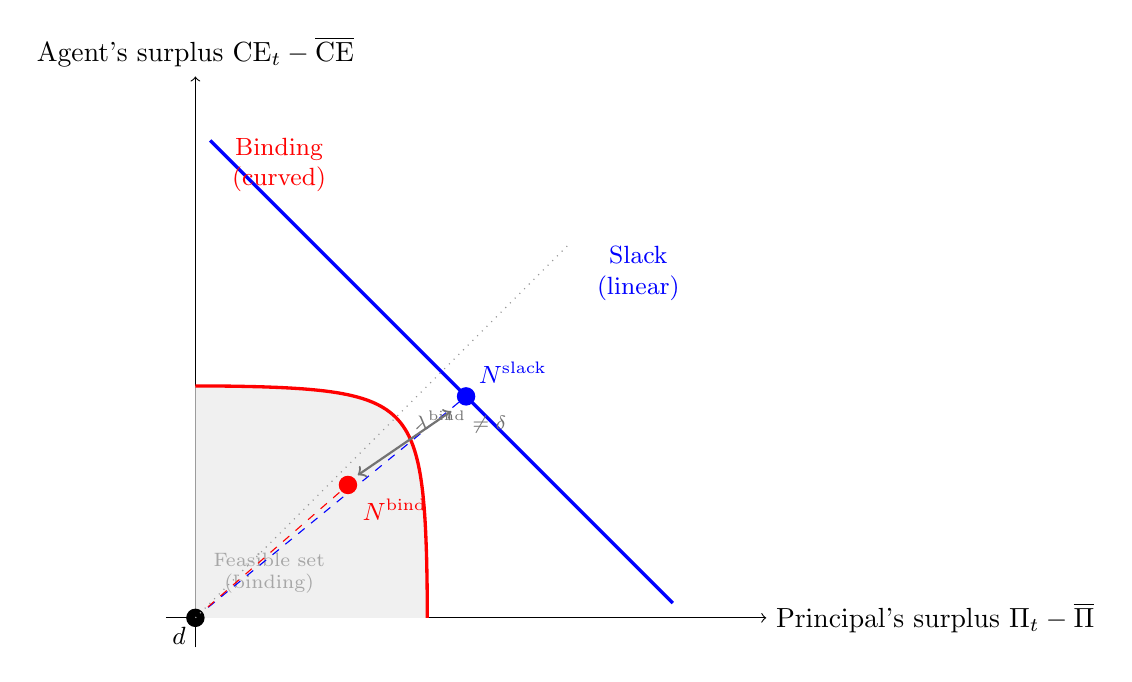
\begin{tikzpicture}[scale=1.25]
    \draw[->] (-0.3,0) -- (5.8,0) node[right] {Principal's surplus $\Pi_t - \overline{\Pi}$};
    \draw[->] (0,-0.3) -- (0,5.5) node[above] {Agent's surplus $\text{CE}_t - \overline{\text{CE}}$};

    \fill[gray!12] plot[domain=0:90, smooth, samples=60]
        ({3.8*sin(\x) * (1 - 0.38*sin(\x)^1.3)},
         {3.8*cos(\x) * (1 - 0.38*cos(\x)^1.3)})
        -- (0,0) -- cycle;
    \node[gray!70, font=\scriptsize, align=center] at (0.75,0.45) {Feasible set\\(binding)};

    \draw[very thick, blue] (0.15,4.85) -- (4.85,0.15);
    \node[blue, font=\small, align=center] at (4.5,3.5) {Slack\\(linear)};

    \filldraw[blue] (2.75,2.25) circle (2.5pt);
    \node[blue, font=\small, above right] at (2.78,2.28) {$N^{\text{slack}}$};
    \draw[dashed, blue, thin] (0,0) -- (2.75,2.25);

    \draw[very thick, red, domain=0:90, smooth, samples=80]
        plot ({3.8*sin(\x) * (1 - 0.38*sin(\x)^1.3)},
             {3.8*cos(\x) * (1 - 0.38*cos(\x)^1.3)});
    \node[red, font=\small, align=center] at (0.85,4.6) {Binding\\(curved)};

    \filldraw[red] (1.55,1.35) circle (2.5pt);
    \node[red, font=\small, right] at (1.6,1.1) {$N^{\text{bind}}$};
    \draw[dashed, red, thin] (0,0) -- (1.55,1.35);

    \filldraw[black] (0,0) circle (2.5pt);
    \node[below left, font=\small] at (0,0) {$d$};

    \draw[<->, thick, black!55] (2.6,2.1) -- (1.65,1.45)
        node[midway, above right, font=\scriptsize] {$\lambda^{\text{bind}} \neq \delta$};

    \draw[dotted, black!40, thin] (0,0) -- (3.8,3.8);

\end{tikzpicture}
\caption*{\textit{Source:} Own elaboration.}
\label{fig:ntu_frontier}
\end{figure}

Since $\underline{w}_t$ depends on wealth through $W_t$, and $\beta_t^*$ depends on $\underline{w}_t$, realized bargaining power $\lambda_t$ becomes history-dependent through the wealth accumulation process. In general, $\lambda_t \neq \delta$ when the constraint binds. When limited liability does not bind, the Pareto frontier is linear and the Nash solution achieves any surplus split by adjusting $\alpha_t$ while keeping efficiency at $\beta^{\text{eff}}$, so $\lambda_t = \delta$ always. When limited liability binds, the constraint pins $\alpha_t$ and the Pareto frontier becomes curved: points corresponding to different wealth levels face different feasible sets, so their realized bargaining power differs even under the same exogenous Nash parameter $\delta$. Moving along the curved frontier requires changing $\beta_t$, which affects total surplus and generates the non-transferability that makes bargaining outcomes history-dependent.

\begin{remark}[Welfare comparison: constrained planner versus Nash equilibrium]\label{rem:welfare}
The binding regime generates a third layer of efficiency loss, on top of the two already identified in Section \ref{subsec:symmetric}. To see this, consider a constrained planner who respects incentive compatibility and limited liability but is not subject to Nash bargaining: the planner maximizes total surplus $S(\beta)$ subject to $\alpha \geq \underline{w}(W) - \beta\underline{y}$.

The planner sets $\alpha = \underline{w}(W) - \beta\underline{y}$ at the boundary (since any slacker $\alpha$ wastes surplus), but is free to choose $\beta$ independently to maximize $S(\beta)$. The limited liability constraint binds only on $\alpha$, not on $\beta$. The planner therefore implements $\beta^{\mathrm{eff}}$ regardless of $W$, achieving $S^{\mathrm{eff}} = S(\beta^{\mathrm{eff}})$ in every period.

The Nash equilibrium in the binding regime instead chooses $\beta^*(W) \neq \beta^{\mathrm{eff}}$, because the parties use $\beta_t$ both to set incentives and to redistribute surplus. The resulting equilibrium surplus is $S(\beta^*(W)) < S(\beta^{\mathrm{eff}})$, since $\beta^{\mathrm{eff}}$ is the unique maximizer of $S(\beta)$. The bargaining distortion is
\[
\Delta(W) := S^{\mathrm{eff}} - S(\beta^*(W)) = \frac{(\beta^{\mathrm{eff}} - \beta^*(W))^2}{2} \left(\frac{\theta^2}{k} + \gamma\sigma^2\right) > 0,
\]
where the equality uses the quadratic form of $S(\beta)$ around its maximum. Three features of $\Delta(W)$ are worth noting. First, $\Delta(W) = 0$ in the slack regime, where $\beta^*(W) = \beta^{\mathrm{eff}}$: bargaining introduces no additional distortion when transfers are unconstrained. Second, $\Delta(W)$ is increasing in $|\beta^*(W) - \beta^{\mathrm{eff}}|$, which is itself increasing in how far $W$ is below $\overline{W}$: poorer agents face tighter constraints, larger distortions in $\beta^*$, and greater welfare losses. Third, $\Delta(W)$ is increasing in $\theta^2/k + \gamma\sigma^2$, the curvature of the surplus function: when the risk-incentive trade-off is steep, small deviations of $\beta^*$ from $\beta^{\mathrm{eff}}$ are more costly.

The full efficiency loss relative to first-best therefore decomposes as
\[
S^{\mathrm{FB}} - S(\beta^*(W)) = \underbrace{(S^{\mathrm{FB}} - S^{\mathrm{eff}})}_{\text{moral hazard}} + \underbrace{\Delta(W)}_{\text{bargaining distortion}},
\]
with the second term present only in the binding regime and vanishing as $W \to \overline{W}$. This decomposition clarifies that policies reducing the stringency of the limited liability constraint (raising $\gamma_w$ or increasing $W$) improve welfare not only by relaxing the constraint directly but also by reducing the bargaining distortion $\Delta(W)$.
\end{remark}
\end{document}
